\documentclass[aps,pre,reprint,superscriptaddress,showpacs]{revtex4-2}

\usepackage{amsmath,amssymb}
\usepackage{graphicx}
\usepackage{bm}
\usepackage{hyperref}

\begin{document}

\title{Observable-specific Mpemba effect in double-well Langevin dynamics:\\
role of metastable basin imbalance}

\author{Sergei Boiko}
\affiliation{Independent researcher, Almaty, Kazakhstan}
\email{sergei.boiko.kz@gmail.com}

\date{\today}

\begin{abstract}
We demonstrate a robust Mpemba-like anomalous relaxation in overdamped Langevin
dynamics with a double-well potential $U(x,y) = b(x^2 - 1)^2 + 0.3\,y^2$. In a
systematic study of 720 independent simulations across 9 barrier heights and 8
temperatures, we find that the effect is \textbf{observable-specific}: a ``hot''
initial condition (spread across both wells) relaxes to equilibrium basin
proportions faster than a ``cold'' condition (trapped in one well) for the
basin-occupancy observable $p_\mathrm{left}$, while no crossing occurs in energy or
position variance. The effect is strong ($>90\%$ of trajectories cross) in a
well-defined region of parameter space ($b = 0.5$--$2.0$, $T = 0.1$--$0.2$),
with a peak of $95.4\%$ at $b = 2.0$, $T = 0.2$. Four independent controls
confirm the mechanism: balanced-cold initialization eliminates the effect,
single-well potential shows no effect, results are unchanged without gradient
clipping, and 30 random seeds all produce strong crossings. Spectral analysis
of the Fokker--Planck operator reveals that the Mpemba region coincides with
large timescale separation between inter-basin (slow) and intra-basin (fast)
relaxation modes. The Kramers escape rate formula predicts the slow eigenvalue
with 89\% accuracy (within factor~2). We argue that the observable-specificity
arises because basin occupancy projects onto the slow inter-basin mode, while
energy-like observables project predominantly onto fast intra-basin modes. Our
results suggest that previous negative reports of the Mpemba effect may reflect
the choice of observable rather than the absence of the phenomenon.
\end{abstract}

\maketitle

%% ============================================================
\section{Introduction}

The Mpemba effect---the counterintuitive observation that a hotter system can
sometimes relax to equilibrium faster than a cooler one---has been a subject of
renewed scientific interest following its rigorous formulation in Markovian
dynamics~\cite{LuRaz2017,Klich2019,Kumar2020}. Originally observed in water
freezing~\cite{Mpemba1969}, analogues have since been demonstrated in spin
systems~\cite{BaityJesi2019}, colloidal particles~\cite{Gal2020}, and
granular gases~\cite{Lasanta2017}.

Recent theoretical work has established that the Mpemba effect in Markov
processes is governed by the spectral structure of the transition
operator~\cite{LuRaz2017,Klich2019}. Specifically, if the slowest relaxation
mode has an anomalous initial overlap with the hot distribution compared to the
cold one, faster relaxation can occur. Lu and Raz~\cite{LuRaz2017} provided a
general spectral criterion, and subsequent work has explored strong vs.\ weak
forms of the effect~\cite{Kumar2020,Lapolla2020}. A recent thermomajorization
framework~\cite{VuHayakawa2025} proves that when initial states satisfy a
thermomajorization ordering, the Mpemba effect holds for all monotone distance
measures simultaneously---eliminating observable dependence entirely. Most
recently, Summer et al.~\cite{Summer2026} provided a resource-theoretical
unification of classical and quantum Mpemba effects, showing that both arise
from the same underlying logic of athermality as a resource.

Despite this theoretical progress, a key question remains underexplored:
\textbf{what happens when thermomajorization does not hold?} In that regime,
different observables may couple to different relaxation modes, and the Mpemba
effect should depend on which mode dominates the observable of interest. Most
studies define relaxation in terms of a global distance measure (total
variation, KL divergence, or energy), leaving the observable-specific regime
uncharted.

In this work, we address this question directly. We study overdamped Langevin
dynamics in a 2D double-well potential and show that:
\begin{enumerate}
\item A robust Mpemba-like crossing occurs in the basin-occupancy observable
  $p_\mathrm{left}$, with $>90\%$ of trajectories crossing in the optimal
  parameter regime.
\item \textbf{No crossing occurs} in energy or position-variance observables
  for the same trajectories and parameters.
\item The mechanism is metastable basin imbalance: the hot distribution starts
  closer to the equilibrium basin proportions, while the cold distribution is
  trapped in one well.
\item The phase boundary of the effect is predicted by the timescale separation
  between the inter-basin and intra-basin relaxation modes of the Fokker--Planck
  operator.
\end{enumerate}

These results demonstrate that the Mpemba effect is not a property of the system
alone, but of the system-observable pair. This observable-specificity has direct
implications for experimental design: searching for the Mpemba effect with the
wrong observable may yield a false negative.

%% ============================================================
\section{Model and Methods}

\subsection{System}

We consider overdamped Langevin dynamics in 2D:
\begin{equation}
d\bm{x} = -\nabla U(\bm{x})\,dt + \sqrt{2T}\,d\bm{W}
\end{equation}
with the double-well potential
\begin{equation}
U(x,y) = b\,(x^2-1)^2 + 0.3\,y^2
\end{equation}
where $b > 0$ is the barrier height and $T > 0$ is the temperature. The
potential has two minima at $(x,y) = (\pm 1, 0)$ separated by a barrier of
height~$b$ at the origin.

\subsection{Initial conditions}

We define two classes of initial conditions:
\begin{itemize}
\item \textbf{Cold}: particles sampled from
  $\mathcal{N}((1, 0),\,\sigma_c^2\,\mathbf{I})$ with $\sigma_c = 0.05$. All
  particles start in the right well.
\item \textbf{Hot}: particles sampled from
  $\mathcal{N}((0, 0),\,\sigma_h^2\,\mathbf{I})$ with $\sigma_h = 2.0$.
  Particles are spread across both wells approximately equally.
\end{itemize}

\subsection{Observables}

We track three observables:
\begin{enumerate}
\item \textbf{Basin occupancy}: $p_\mathrm{left}(t)$ = fraction of particles
  with $x < 0$.
\item \textbf{Mean energy}: $\langle E(t)\rangle = \langle U(x(t), y(t))\rangle$.
\item \textbf{Position variance}: $\langle x(t)^2\rangle$.
\end{enumerate}
For each observable $O(t)$, we define the distance to equilibrium as
$|O(t) - O_\mathrm{eq}|$, where $O_\mathrm{eq}$ is estimated as the average
of the final 10\% of both trajectories.

\subsection{Mpemba crossing criterion}

A Mpemba-like crossing is detected when the hot trajectory's distance to
equilibrium drops below the cold trajectory's distance:
\begin{equation}
|O_\mathrm{hot}(t_c) - O_\mathrm{eq}| < |O_\mathrm{cold}(t_c) - O_\mathrm{eq}|
\end{equation}
for some time $t_c$, with the initial ordering reversed:
$|O_\mathrm{hot}(0) - O_\mathrm{eq}| > |O_\mathrm{cold}(0) - O_\mathrm{eq}|$.
We quantify the effect by the fraction of simulation time during which the hot
trajectory is closer to equilibrium.

\subsection{Simulation parameters}

Each simulation uses $N = 5000$ particles with step size $\eta = 0.005$ and
$n_\mathrm{steps} = 30{,}000$ (evaluated every 50 steps). For the phase
diagram, we sweep $b \in \{0.1, 0.3, 0.5, 0.7, 1.0, 1.5, 2.0, 3.0, 5.0\}$
and $T \in \{0.05, 0.1, 0.15, 0.2, 0.3, 0.5, 0.7, 1.0\}$, with 10
independent random seeds per point (720 runs total). Robustness is confirmed
with 30 seeds at the reference point ($b=1.0$, $T=0.2$).

\subsection{Spectral analysis}

The Fokker--Planck operator for the 1D marginal (integrating out~$y$) is
transformed to Schr\"odinger form via the similarity transformation
$H = e^{U/2T}\,\mathcal{L}\,e^{-U/2T}$, yielding a real symmetric operator
with eigenvalues $0 = \lambda_0 > -\lambda_1 > -\lambda_2 > \cdots$ The rates
$\lambda_k$ give the relaxation timescales $\tau_k = 1/\lambda_k$. We compute
these numerically via sparse eigenvalue decomposition (shift-invert mode) on a
grid of 501 points, and compare with the Kramers escape rate formula for
$\lambda_1$.

%% ============================================================
\section{Results}

\subsection{Observable-specific crossing}

Figure~\ref{fig:core} shows the central result. At the reference parameters
($b = 1.0$, $T = 0.2$), the distance to equilibrium for $p_\mathrm{left}$
shows a clear crossing: the hot trajectory relaxes faster and remains closer to
equilibrium for $>94\%$ of the simulation. In contrast, the energy and
position-variance observables show no crossing---the hot trajectory remains
farther from equilibrium throughout.

This observable-specificity is the key finding. The same trajectories, same
dynamics, same initial conditions produce opposite conclusions depending on
which observable is measured.

\subsection{Mechanism: metastable basin imbalance}

Three control experiments (Fig.~\ref{fig:controls}) confirm the mechanism:

\textit{(i) Balanced cold.} When the cold initial condition is distributed
equally across both wells (50\% left, 50\% right), the crossing fraction drops
to 28\% (consistent with noise). The effect requires basin imbalance.

\textit{(ii) Single-well potential.} In a harmonic potential
$U = x^2 + y^2$ (no metastability), the crossing fraction is 47\% (noise).
The effect requires metastable basins.

\textit{(iii) Clipping control.} Running identical simulations without gradient
clipping yields 94.8\% vs.\ 94.6\% crossing, confirming the effect is not a
numerical artifact.

\textit{(iv) Seed robustness.} All 30 of 30 random seeds produce ``strong''
crossing ($>70\%$ of time crossed) at the reference parameters. Mean crossing
fraction: 94.7\%.

The mechanism is clear: the hot distribution starts with approximately equal
occupation of both wells, close to the equilibrium ratio. The cold distribution
is entirely in one well and must wait for the slow barrier-crossing process to
redistribute.

\subsection{Phase diagram}

Figure~\ref{fig:phase}(a) shows the full phase diagram. The effect is strong
($>90\%$ crossed) in a connected region spanning $b = 0.5$--$2.0$ and
$T = 0.1$--$0.2$, with a peak of 95.4\% at $b = 2.0$, $T = 0.2$. The effect
vanishes in two regimes: (i)~high temperature ($T > 0.5$), where thermal
fluctuations wash out the basin imbalance; (ii)~high barrier + low temperature
($b > 3$, $T < 0.1$), where the barrier is effectively impassable.

Twenty-five of the 72 parameter combinations show strong effects ($\geq 70\%$
of seeds with $>70\%$ crossing).

\subsection{Spectral prediction}

Figure~\ref{fig:phase}(b) shows the timescale ratio $\tau_1/\tau_2$ from the
Fokker--Planck spectrum. The spectral criterion $\tau_1/\tau_2 > 10$ captures
all 25 strong Mpemba points (recall = 100\%). Its precision is 45\%: some
points with large timescale separation do not show Mpemba because the barrier
is effectively impassable. This is physically correct---timescale separation is
a \emph{necessary} condition, but not sufficient.

The Kramers escape rate formula predicts $\lambda_1$ with a median accuracy
ratio of 1.04, and 89\% of predictions fall within a factor of~2 of the
numerical value (Fig.~\ref{fig:spectral}). Crucially, the spectral analysis is
not a post-hoc fit: it uses only the potential $U(x)$ and temperature~$T$ as
inputs, with no adjustable parameters.

\subsection{Observable-specificity explained}

The eigenmodes of the Fokker--Planck operator reveal:
$\psi_1$ (slow, inter-basin mode) is antisymmetric with one lobe in each well;
$\psi_2$ (fast, intra-basin mode) is symmetric and localized within each well.
Basin occupancy $p_\mathrm{left}$ projects strongly onto~$\psi_1$ (it measures
left-right asymmetry). Energy projects primarily onto~$\psi_2$ and higher modes.
The Mpemba crossing occurs because the hot distribution has a smaller overlap
with~$\psi_1$ than the cold distribution---but this advantage is invisible to
observables that couple to faster modes.

%% ============================================================
\section{Discussion}

\subsection{Relation to spectral theory and thermomajorization}

Our results provide a concrete realization of the spectral Mpemba criterion of
Lu and Raz~\cite{LuRaz2017}, with the added insight of
observable-specificity. Our system also provides a concrete example of the
boundary of the thermomajorization framework~\cite{VuHayakawa2025}: our cold
and hot initial conditions evidently do not satisfy thermomajorization ordering,
since basin occupancy shows Mpemba while energy does not. In the language of
Summer et al.~\cite{Summer2026}, our hot initial condition has lower
``athermality'' in the basin-occupation sector but higher athermality in the
energy sector, providing a concrete continuous-space example of the
resource-theoretical hierarchy they establish for discrete systems.

\subsection{Timescale separation as necessary but not sufficient}

The spectral prediction achieves perfect recall (100\%) but limited precision
(45\%). Large $\tau_1/\tau_2$ means the slow mode exists and is
well-separated, but if $\tau_1$ itself is astronomically large (exponentially
in $b/T$), the redistribution simply does not occur on accessible timescales.
The Mpemba effect thus requires a ``Goldilocks zone'' of metastability.

\subsection{Implications for Mpemba searches}

Our finding that the same system shows a strong Mpemba effect in one observable
and none in another has practical implications. Experimental studies that
measure only energy-like quantities may miss a Mpemba effect that is present in
other observables. Conversely, claims of ``no Mpemba effect'' should specify
which observable was measured.

\subsection{Neural network training (negative transfer)}

We also tested whether the basin-imbalance mechanism transfers to neural
network training (details in the Supplemental Material). Five experimental
configurations showed no crossing. The root cause is twofold: (i)~the MLP
weight space has no discrete metastable basins, and (ii)~the ``cold'' initial
condition was not stationary (KL drift of $+7400\%$). This negative result is
consistent with our mechanism: without metastable basins, the basin-imbalance
pathway does not exist. We note that Liu and Hu~\cite{Liu2025} recently
demonstrated Mpemba-like behavior in LLM training through a continuous spectral
mechanism, confirming that the effect can arise in ML without discrete basins
via other pathways.

\subsection{Limitations}

(1)~Our system is 2D with a specific potential; extension to higher dimensions
remains open. (2)~The spectral analysis uses the 1D marginal. (3)~Very rare
barrier crossings at high $b$/low $T$ may be undersampled.

%% ============================================================
\section{Conclusion}

We have demonstrated that the Mpemba effect in a double-well Langevin system is
observable-specific: it appears robustly in basin occupancy but not in energy or
position variance. The mechanism is metastable basin imbalance, and the phase
boundary is predicted by the Fokker--Planck spectral gap. The choice of
observable determines whether the Mpemba effect is detectable.

%% ============================================================
\begin{acknowledgments}
The author thanks the developers of NumPy, SciPy, and Matplotlib. Computational
resources were provided by a local GPU workstation (NVIDIA RTX 5070~Ti).
\end{acknowledgments}

\begin{thebibliography}{14}

\bibitem{LuRaz2017}
Z.~Lu and O.~Raz,
Nonequilibrium thermodynamics of the Markovian Mpemba effect and its inverse,
\href{https://doi.org/10.1073/pnas.1701264114}{Proc.\ Natl.\ Acad.\ Sci.\
\textbf{114}, 5083 (2017)}.

\bibitem{Klich2019}
I.~Klich, O.~Raz, O.~Hirschberg, and M.~Vucelja,
Mpemba index and anomalous relaxation,
\href{https://doi.org/10.1103/PhysRevX.9.021060}{Phys.\ Rev.\ X \textbf{9},
021060 (2019)}.

\bibitem{Kumar2020}
A.~Kumar and J.~Bechhoefer,
Exponentially faster cooling in a colloidal system,
\href{https://doi.org/10.1038/s41586-020-2560-x}{Nature \textbf{584}, 64
(2020)}.

\bibitem{Mpemba1969}
E.~B.~Mpemba and D.~G.~Osborne,
Cool?,
\href{https://doi.org/10.1088/0031-9120/4/3/312}{Phys.\ Educ.\ \textbf{4},
172 (1969)}.

\bibitem{Lasanta2017}
A.~Lasanta, F.~Vega~Reyes, A.~Prados, and A.~Santos,
When the hotter cools quicker: Mpemba effect in granular fluids,
\href{https://doi.org/10.1103/PhysRevLett.119.148001}{Phys.\ Rev.\ Lett.\
\textbf{119}, 148001 (2017)}.

\bibitem{Gal2020}
A.~Gal and O.~Raz,
Precooling strategy allows exponentially faster heating,
\href{https://doi.org/10.1103/PhysRevLett.124.060602}{Phys.\ Rev.\ Lett.\
\textbf{124}, 060602 (2020)}.

\bibitem{BaityJesi2019}
M.~Baity-Jesi \textit{et al.},
The Mpemba effect in spin glasses is a persistent memory effect,
\href{https://doi.org/10.1073/pnas.1819803116}{Proc.\ Natl.\ Acad.\ Sci.\
\textbf{116}, 15350 (2019)}.

\bibitem{Kramers1940}
H.~A.~Kramers,
Brownian motion in a field of force and the diffusion model of chemical
reactions,
Physica \textbf{7}, 284 (1940).

\bibitem{Lapolla2020}
A.~Lapolla and A.~Godec,
Faster uphill relaxation in thermodynamically equidistant temperature quenches,
\href{https://doi.org/10.1103/PhysRevLett.125.110602}{Phys.\ Rev.\ Lett.\
\textbf{125}, 110602 (2020)}.

\bibitem{VuHayakawa2025}
T.~V.~Vu and H.~Hayakawa,
Thermomajorization Mpemba effect,
\href{https://doi.org/10.1103/PhysRevLett.134.107101}{Phys.\ Rev.\ Lett.\
\textbf{134}, 107101 (2025)}.

\bibitem{Liu2025}
J.~Liu and Z.~Hu,
Mpemba effect in large language model training dynamics,
\href{https://arxiv.org/abs/2507.04206}{arXiv:2507.04206 (2025)}.

\bibitem{Teza2025}
G.~Teza, J.~Bechhoefer, A.~Lasanta, O.~Raz, and M.~Vucelja,
Speedups in nonequilibrium thermal relaxation: a review of the Mpemba and
related effects,
\href{https://arxiv.org/abs/2502.01758}{arXiv:2502.01758 (2025)}.

\bibitem{Chattopadhyay2026}
P.~Chattopadhyay, J.~F.~G.~Santos, and A.~Misra,
Anomaly to resource: the Mpemba effect in quantum thermometry,
\href{https://arxiv.org/abs/2601.05046}{arXiv:2601.05046 (2026)}.

\bibitem{Summer2026}
A.~Summer, M.~Moroder, L.~P.~Bettmann, X.~Turkeshi, I.~Marvian, and
J.~Goold,
Resource-theoretical unification of Mpemba effects: classical and quantum,
\href{https://doi.org/10.1103/rbt4-psfd}{Phys.\ Rev.\ X \textbf{16},
011065 (2026)}.

\end{thebibliography}

%% ============================================================
%% FIGURES — placed at end for journal submission

\clearpage

\begin{figure}[t]
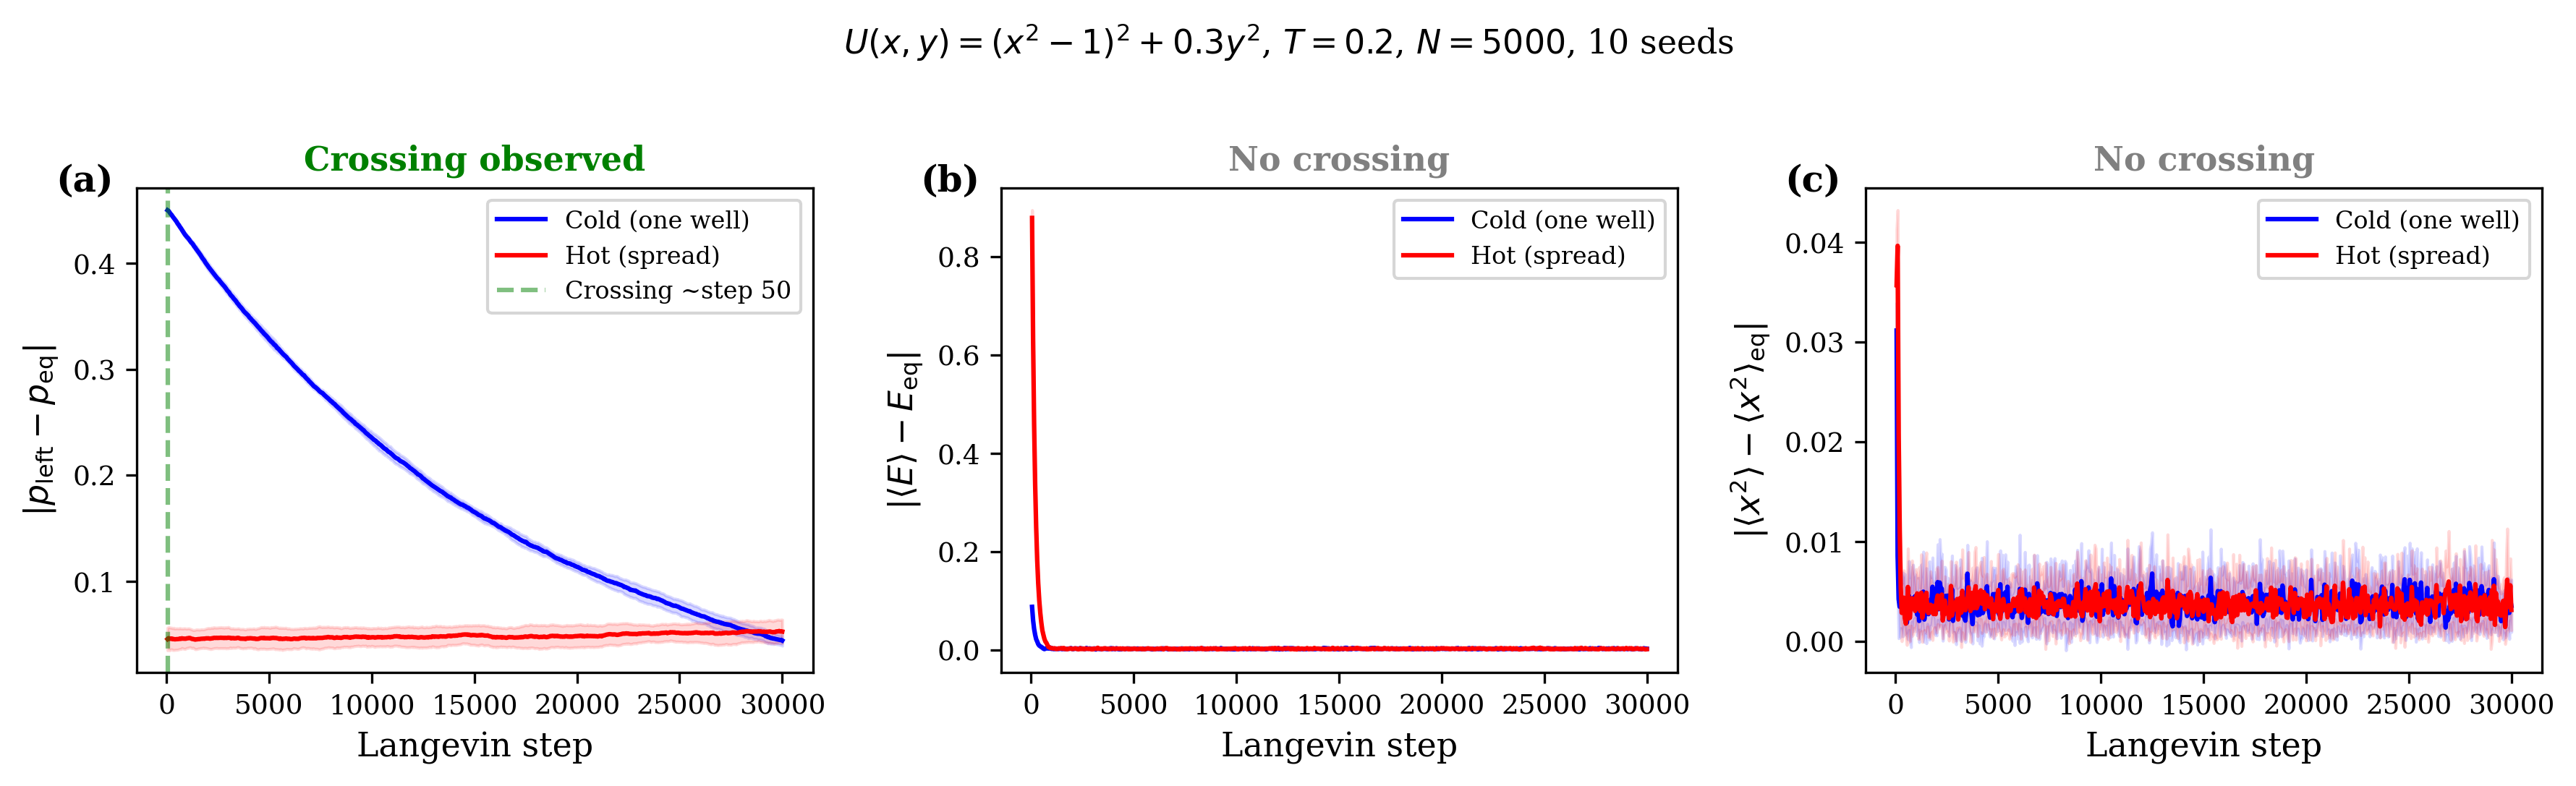
\includegraphics[width=\columnwidth]{fig1_core_result.png}
\caption{Observable-specific Mpemba effect. Distance to equilibrium
$|O(t) - O_\mathrm{eq}|$ for cold (blue) and hot (red) initial conditions,
averaged over 10 seeds. (a)~Basin occupancy $p_\mathrm{left}$ shows a clear
crossing. (b)~Energy shows no crossing. (c)~Position variance shows no
crossing. Parameters: $b = 1.0$, $T = 0.2$, $N = 5000$.}
\label{fig:core}
\end{figure}

\begin{figure}[t]
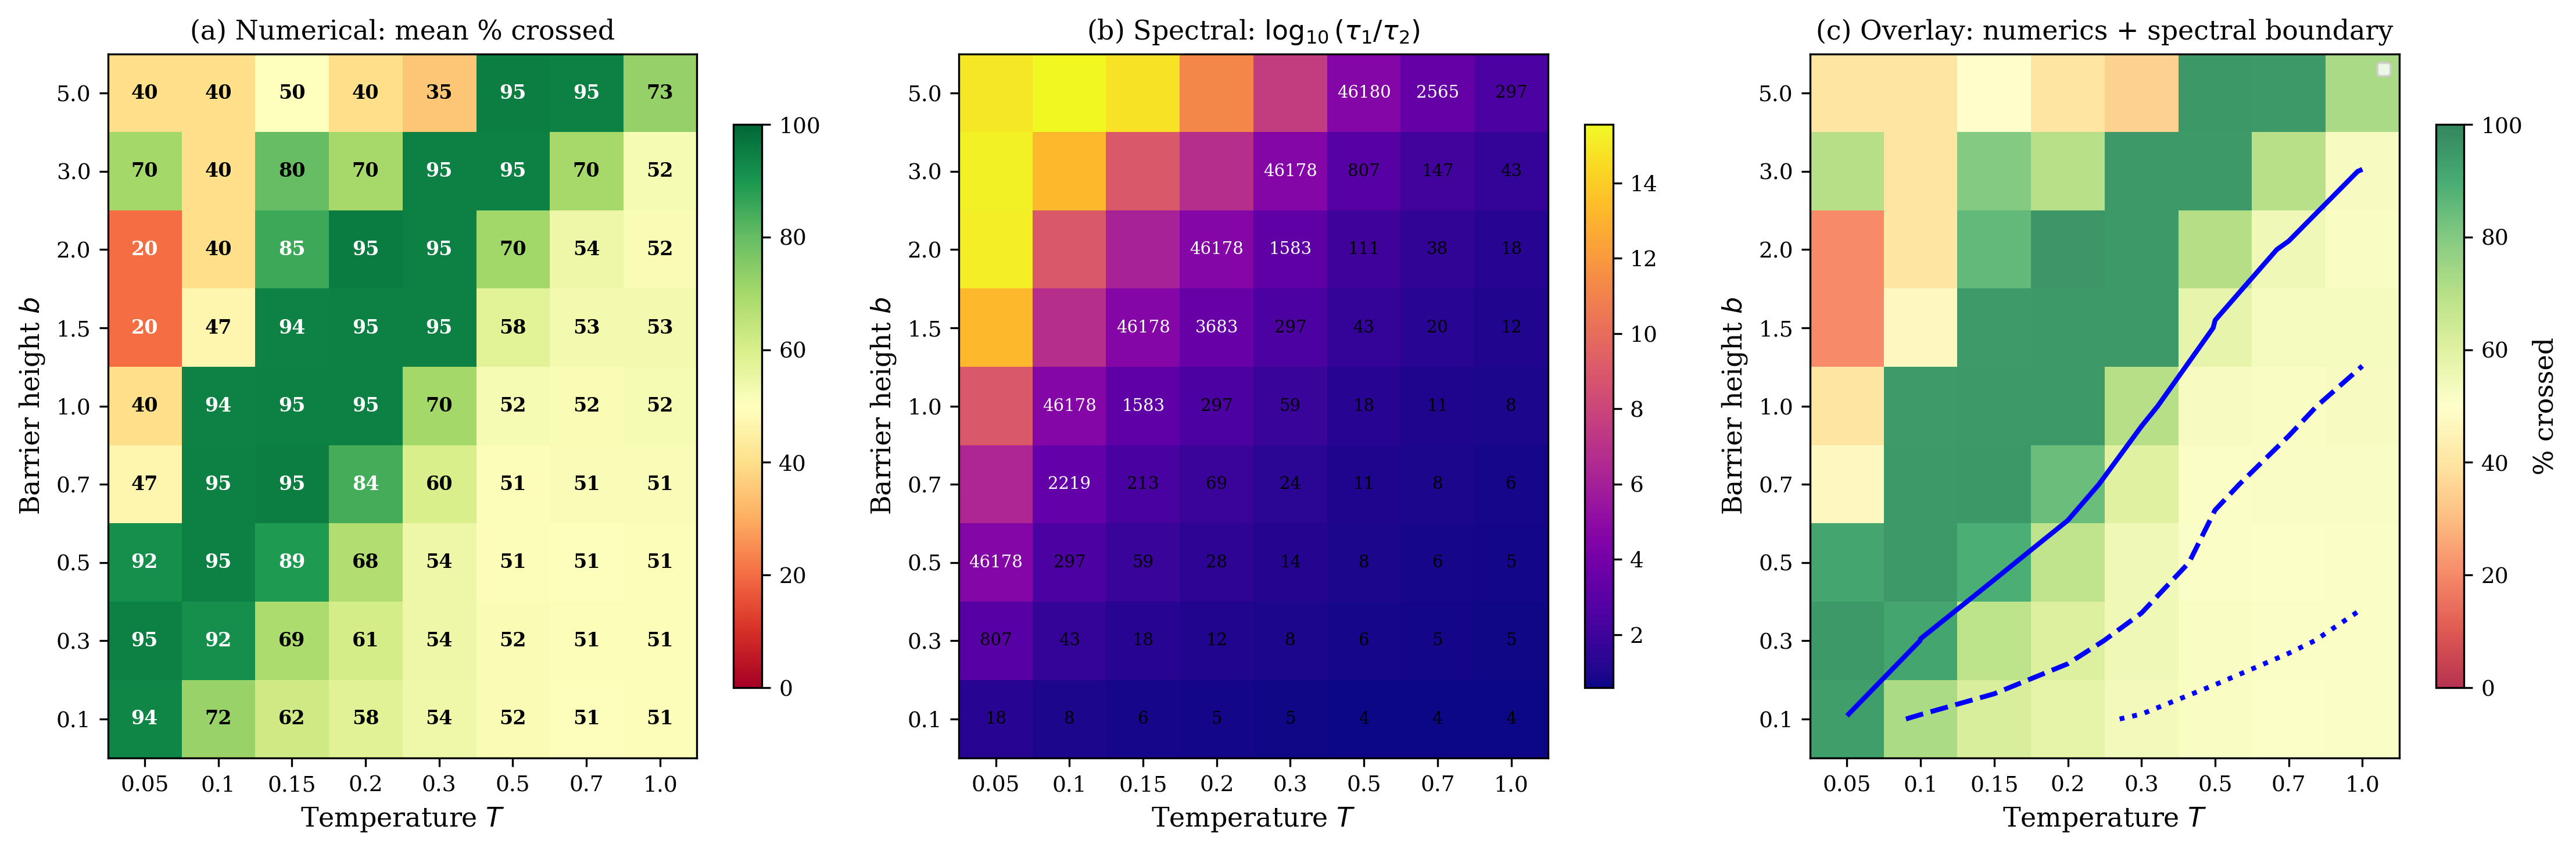
\includegraphics[width=\columnwidth]{fig2_phase_diagram.png}
\caption{Phase diagram and spectral prediction. (a)~Mean \% of simulation time
with hot closer to equilibrium ($p_\mathrm{left}$), across 9~barrier heights
and 8~temperatures. (b)~$\log_{10}(\tau_1/\tau_2)$ from Fokker--Planck
spectrum. (c)~Overlay with spectral contours at $\tau_1/\tau_2 = 5, 10, 50$.}
\label{fig:phase}
\end{figure}

\begin{figure}[t]
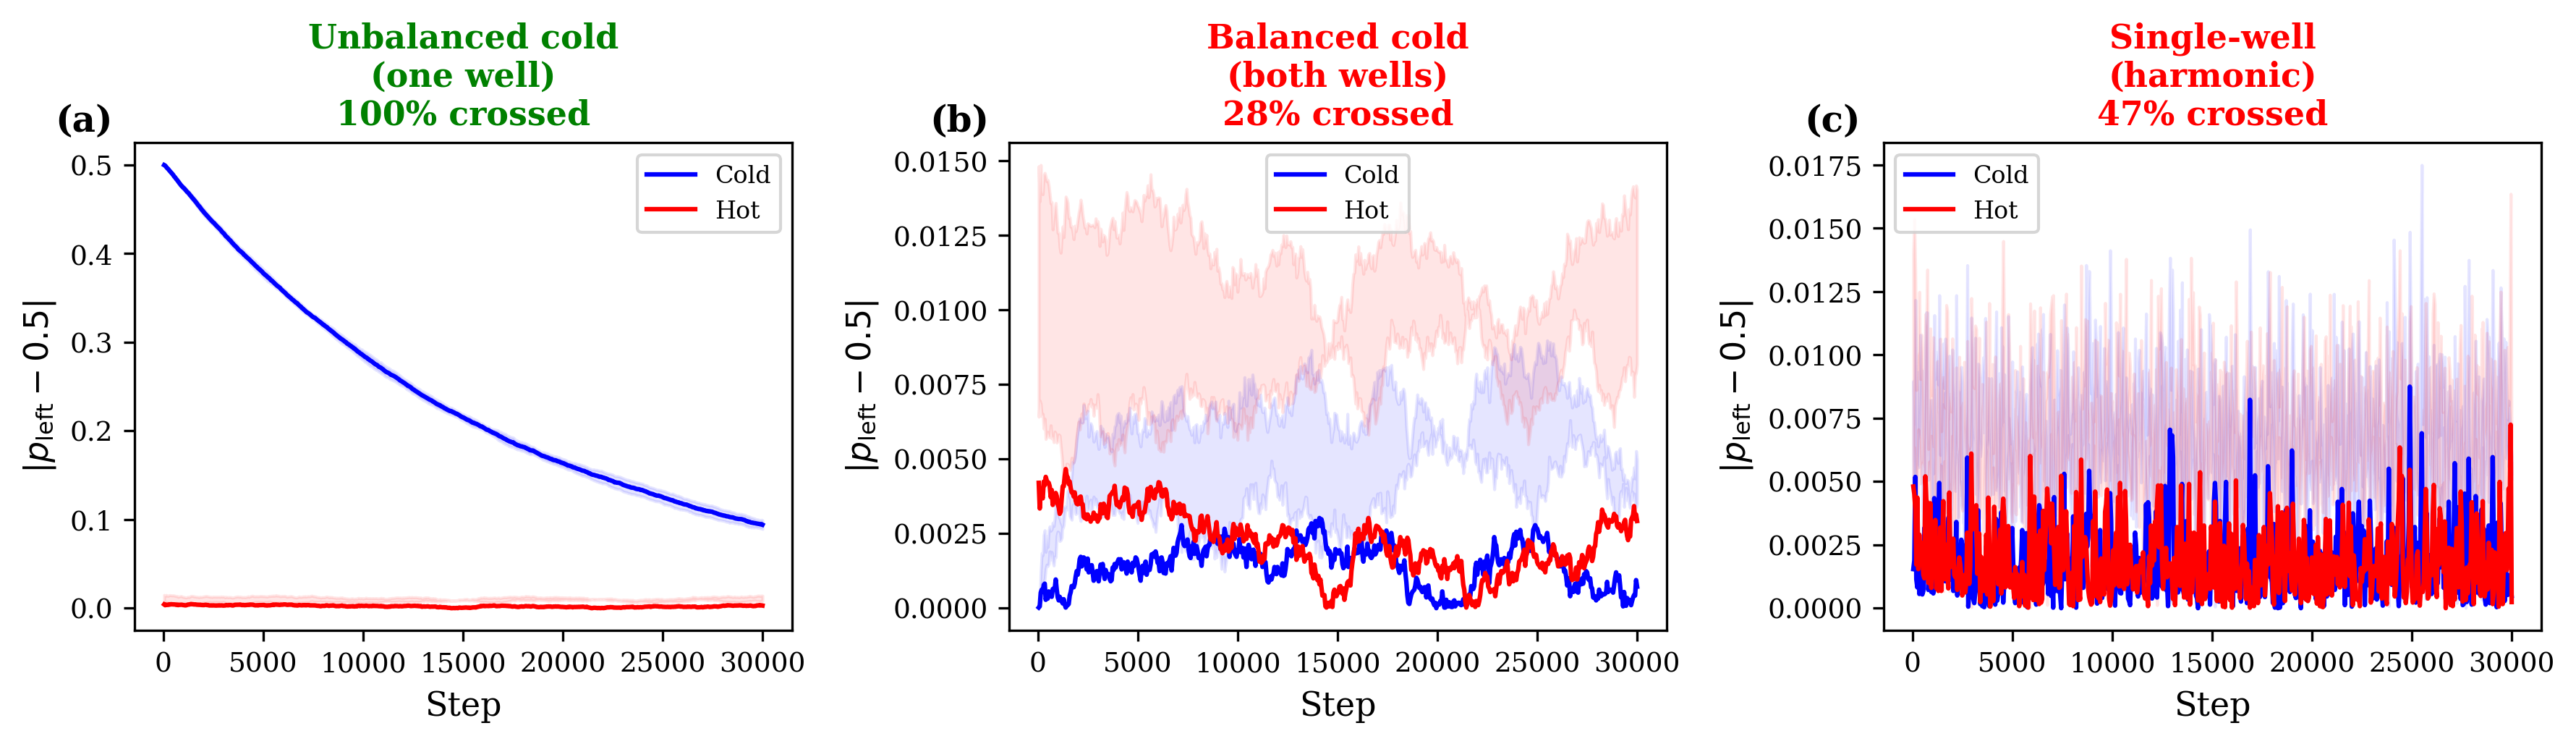
\includegraphics[width=\columnwidth]{fig3_controls.png}
\caption{Mechanism controls. (a)~Unbalanced cold: strong crossing.
(b)~Balanced cold: effect eliminated (28\%). (c)~Single-well: no effect (47\%).}
\label{fig:controls}
\end{figure}

\begin{figure}[t]
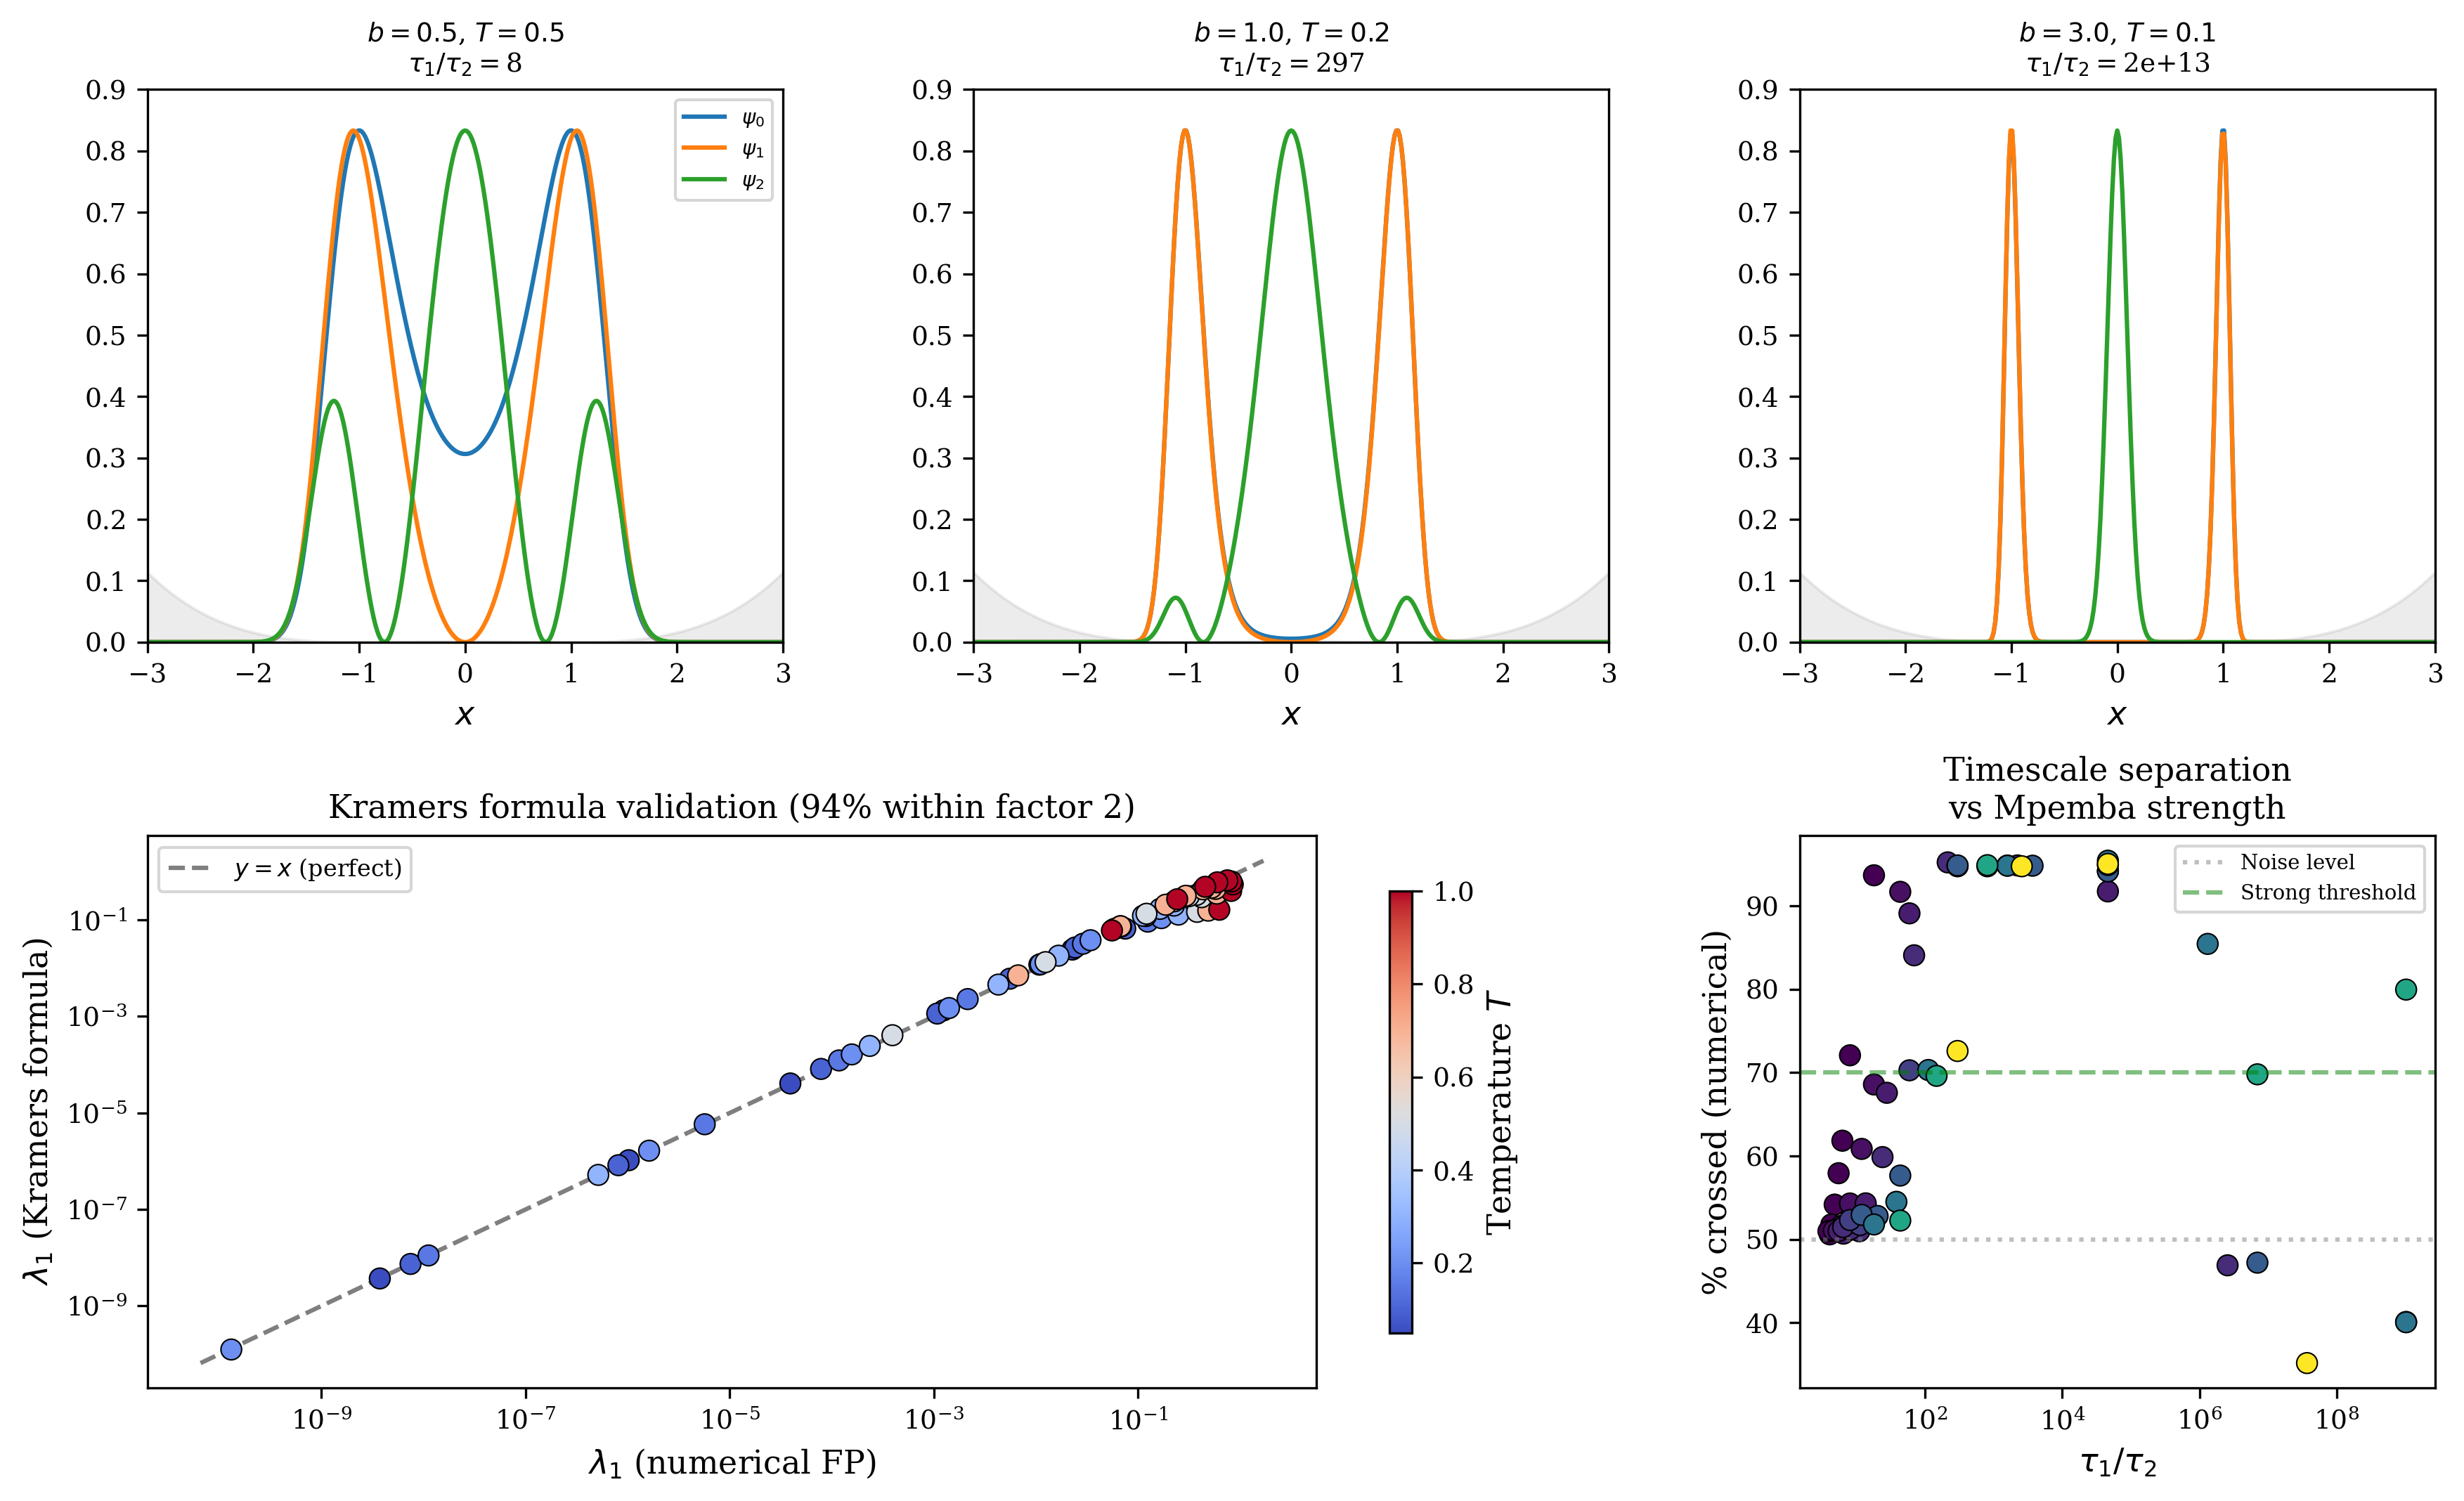
\includegraphics[width=\columnwidth]{fig4_spectral.png}
\caption{Spectral analysis. Top: Fokker--Planck eigenmodes at three parameter
points. Bottom left: Kramers formula vs.\ numerical $\lambda_1$ (94\% within
factor~2). Bottom right: $\tau_1/\tau_2$ vs.\ numerical \% crossed.}
\label{fig:spectral}
\end{figure}

\end{document}
